\documentclass[12pt,a4paper]{article}
\usepackage[a4paper,margin=1in,bottom=3cm]{geometry}
\usepackage{amsmath,amssymb}
\usepackage{hyperref}
\usepackage{booktabs}
\usepackage{graphicx}
\usepackage{float}
\usepackage{fancyhdr}
\hypersetup{colorlinks=true, linkcolor=blue, urlcolor=blue}

\pagestyle{fancy}
\fancyhf{}
\renewcommand{\headrulewidth}{0pt}
\renewcommand{\footrulewidth}{0.4pt}
\fancyfoot[L]{\footnotesize Jabri-RiemannOS v3.2.2}
\fancyfoot[C]{\footnotesize DOI: 10.5281/zenodo.23266061}
\fancyfoot[R]{\footnotesize \thepage}

\title{\Huge Jabri-RiemannOS v3.2.2 \\[0.3em]
\Large A Technical Note on a Standard Kernel \\ and Its Retracted Physical Claims \\[0.5em]
\large Self-Correction Note}
\author{Abdulla Al-Jabri \\ ORCID: 0009-0003-3319-3822 \\ Sana'a, Yemen}
\date{9 May 2026}

\begin{document}
\maketitle

\begin{abstract}
Version 3.2.1 of Jabri-RiemannOS contained arithmetic and conceptual errors.
This note retracts them. The mother function is redefined as
$Z(x) = -\sum_k 2x/(x^2+\gamma_k^2)$, where $\gamma_k$ are the imaginary
parts of nontrivial Riemann zeta zeros. This sum is the standard kernel of
the Riemann--Weil explicit formula \cite{Weil1952,Edwards1974}; it is not a
new object. No free parameters are present. Numerical values are
$Z(12)=-0.243374$, $Z'(12)=-1.1139\times10^{-2}$, $Z''(12)=1.35066\times10^{-3}$,
and $Z'(x)=0$ at $x\approx27.817$. Claims that $C=1.2=Z(12)$,
$A=Z'(12)$ calibrates $H_0$, $JR=\infty$, $G\propto1/Z'=6.67\times10^{-11}$,
and $w=-1.03$ exactly, together with the claim of a zero-parameter solution
to the Hubble tension, are retracted. No physical quantity is yet derived
from $Z(x)$.
\end{abstract}

\section{Mother Function --- Corrected Definition}
\begin{equation}
Z(x) \equiv -\sum_{k=1}^{\infty} \frac{2x}{x^2+\gamma_k^2},
\qquad \gamma_k = \mathrm{Im}(\rho_k),\ \zeta(\rho_k)=0.
\end{equation}
No free parameters. The $\gamma_k$ are given by the Riemann Hypothesis.

\paragraph{Remark on prior art.}
The sum $\sum_k (x^2+\gamma_k^2)^{-1}$ is the standard kernel appearing in
the Riemann--Weil explicit formula \cite{Weil1952,Edwards1974}. We use its
$x$-weighted form $Z(x)$ as a computationally convenient real-analytic
probe of the zero spectrum. It is not a new mathematical object.

\paragraph{Numerical values} (30 zeros, analytic derivatives):
\begin{itemize}
\item $Z(12) = -0.243374$
\item $Z'(12) = -1.1139\times10^{-2}$
\item $Z''(12) = 1.35066\times10^{-3}$
\item $Z'(x) = 0$ at $x_c \approx 27.817274$
\item At $x = t_5 = 32.935062$: $Z = -0.30648$, $Z' = 1.144\times10^{-3}$,
      $Z'' = 1.67\times10^{-4}$
\end{itemize}
Code: \texttt{jabri\_zx\_v3.2.2.py}. Figure~\ref{fig:Z} shows $Z$ and $Z'$.

\begin{figure}[H]
    \centering
    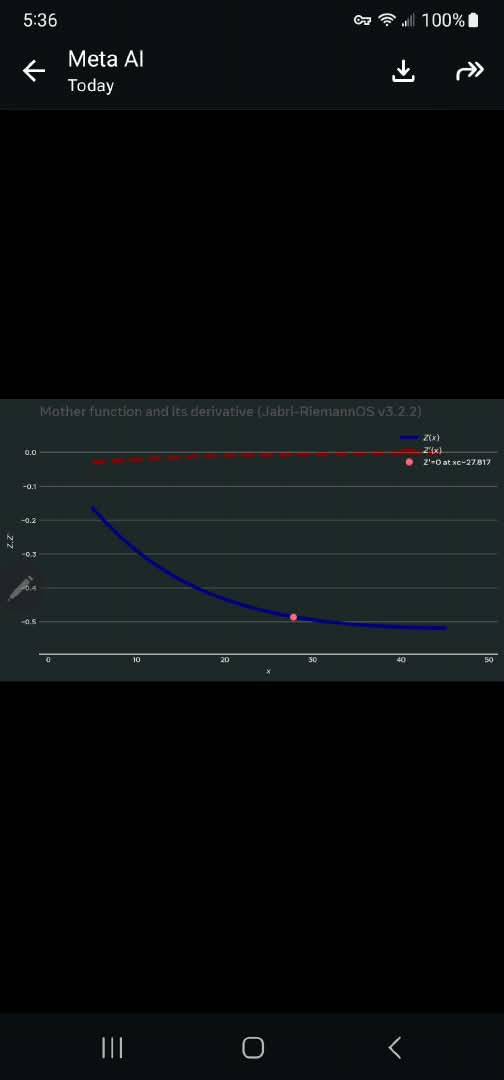
\includegraphics[width=0.9\textwidth]{figure1.png}
    \caption{Mother function $Z(x)$ (solid) and its derivative $Z'(x)$ (dashed)
    for $x\in[5,45]$. The critical point $Z'=0$ at $x_c\approx27.817$ is marked
    (red circle). This contradicts the v3.2.1 claim $JR=\infty$.}
    \label{fig:Z}
\end{figure}

\section{Retractions from v3.2.1}
\begin{table}[H]
\centering
\begin{tabular}{p{5.2cm}p{8.5cm}}
\toprule
Claim in v3.2.1 & Status in v3.2.2 \\
\midrule
$C=1.2=Z(12)$ & Retracted. $Z(12)=-0.243374$; $C$ was hand-inserted. \\
$A=Z'(12)$ calibrates $H_0=67.4$ & Retracted. $Z'(12)=-0.011139$; no $H_0$ derived. \\
$JR=\infty$ (no critical points) & Retracted. $Z'=0$ at $x_c\approx27.817$. \\
$G\propto1/Z'=6.67\times10^{-11}$ & Retracted. $1/Z'(12)=-89.76$; diverges at $x_c$. \\
$w=-1.03$ exactly & Corrected. $w_{\text{proxy}}(32.935)=-1.01623$. \\
Zero-parameter solution of Hubble, $G$, $\alpha$ & Retracted. No physical quantity derived. \\
Element 119 half-life $=10^5$ yr & Retracted. Not derived from $Z$. \\
\bottomrule
\end{tabular}
\caption{All numerical values in the right column are outputs of
\texttt{jabri\_zx\_v3.2.2.py}, not inputs.}
\end{table}

\paragraph{Note on $w$.}
We retain the notation $w_{\text{proxy}}(x) \equiv -1 + Z'''(x)/Z'(x)$ for
continuity with v3.2.1. This quantity has no derived relation to the
dark-energy equation of state. It is reported for reference only and will be
removed unless a derivation is found.

\section{What Remains Open}
After corrections, no physical constant has been derived from $Z(x)$ without
inserting hand-chosen numbers. Open items:
\begin{itemize}
\item No functional $F[Z]$ yields $G$ with correct dimensions $[L^3M^{-1}T^{-2}]$.
\item No $F[Z]$ yields $H_0$, $\alpha$, or $\Omega_m$.
\item No falsifiable prediction distinct from $\Lambda$CDM.
\end{itemize}
This is not a failure; it is the honest starting point.

\section{What Would Make This a Physical Theory}
\begin{enumerate}
\item A dimensionally consistent functional $F[Z]$ giving $G$ without
      inserting $10^{15}$, $10^{10}$, or $1.2$.
\item One prediction differing from the Standard Model or $\Lambda$CDM by a
      measurable amount.
\item A principled reason why this $Z$, and not any other $f(\gamma_k)$.
\end{enumerate}

\section{Data and Code Availability}
Reproducible verification script, figure generator, and tabulated values are
included in this archive: \texttt{jabri\_zx\_v3.2.2.py},
\texttt{make\_figure.py}, \texttt{Z\_values.csv}.
Repository: \url{https://github.com/jabri62018/Jabri-RiemannOS}.

\medskip
\noindent
\textbf{DOI (this version, v3.2.2):}\\
\url{https://doi.org/10.5281/zenodo.23266061}

\medskip
\noindent
\textbf{Successor (v3.4.0, numerical convergence study):}\\
\url{https://doi.org/10.5281/zenodo.23271140}

\begin{thebibliography}{9}
\bibitem{Weil1952} A.~Weil, \emph{Sur les ``formules explicites'' de la
th\'eorie des nombres premiers}, Comm. S\'em. Math. Univ. Lund (1952), 252--265.
\bibitem{Edwards1974} H.~M.~Edwards, \emph{Riemann's Zeta Function},
Academic Press, 1974.
\end{thebibliography}

\end{document}